\begin{priprava}{7., 8., 9., 10}{}{Graf linearne funckije}{Funkcija}{frontalna, delo v dvojicah/individualno}{drsnice, projekcija, tabla, računalniki}


    \section{Graf linearne funkcije}

    \noindent
\begin{minipage}[c]{0.67\linewidth}

    % \begin{multicols}{2}
                \textbf{Graf linearne funkcije} $f(x)=kx+n$ je predstavljen kot množica točk 
                $$\Gamma_f=\left\{(x,y)\in\mathbb{R}^2 | y=kx+n\right\}, $$
                kar upodobimo kot \textbf{premico}.

                ~\\
                Premice z enako začetno vrednostjo se sekajo v skupni točki $(0,n)$ na ordinatni osi -- \textbf{šop premic}.
                ~\\
                Premice, ki imajo enak smerni koeficient so vzporedne -- \textbf{snop premic}.


        \end{minipage}
         % no space if you would like to put them side by side
        \begin{minipage}[c]{0.3\linewidth}


            \begin{figure}[H]
                    \begin{tikzpicture}
                    % \clip (0,0) rectangle (14.000000,10.000000);
                    {\footnotesize

                    % Drawing 2D Cartesian system
                    \draw (3.000000,3.000000) node [anchor=north east] { $0$ };%
                    \draw [line width=0.016cm] (3.000000,2.925000) -- (3.000000,3.075000);%
                    \draw (3.700000,3.000000) node [anchor=north] { $1$ };%
                    \draw [line width=0.016cm] (3.700000,2.925000) -- (3.700000,3.075000);%
                    % \draw (4.400000,3.000000) node [anchor=north] { $2$ };%
                    \draw [line width=0.016cm] (4.400000,2.925000) -- (4.400000,3.075000);%
                    % \draw (5.100000,3.000000) node [anchor=north] { $3$ };%
                    \draw [line width=0.016cm] (5.100000,2.925000) -- (5.100000,3.075000);%
                    % \draw (2.300000,3.000000) node [anchor=north] { $-1$ };%
                    \draw [line width=0.016cm] (2.300000,2.925000) -- (2.300000,3.075000);%
                    % \draw (1.600000,3.000000) node [anchor=north] { $-2$ };%
                    \draw [line width=0.016cm] (1.600000,2.925000) -- (1.600000,3.075000);%
                    \draw (3.000000,3.700000) node [anchor=east] { $1$ };%
                    \draw [line width=0.016cm] (2.925000,3.700000) -- (3.075000,3.700000);%
                    % \draw (3.000000,4.400000) node [anchor=east] { $2$ };%
                    \draw [line width=0.016cm] (2.925000,4.400000) -- (3.075000,4.400000);%
                    % \draw (3.000000,5.100000) node [anchor=east] { $3$ };%
                    \draw [line width=0.016cm] (2.925000,5.100000) -- (3.075000,5.100000);%
                    % \draw (3.000000,5.800000) node [anchor=east] { $4$ };%
                    \draw [line width=0.016cm] (2.925000,5.800000) -- (3.075000,5.800000);%
                    % \draw (3.000000,2.300000) node [anchor=east] { $-1$ };%
                    \draw [line width=0.016cm] (2.925000,2.300000) -- (3.075000,2.300000);%
                    % \draw (3.000000,1.600000) node [anchor=east] { $-2$ };%
                    % \draw [line width=0.016cm] (2.925000,1.600000) -- (3.075000,1.600000);%
                    \draw (5.700000,3.000000) node [anchor=north] { $x$ };%
                    \draw (3.000000,6.400000) node [anchor=east] { $y$ };%
                    \draw [line width=0.016cm] (1.200000,3.000000) -- (5.700000,3.000000);%
                    \draw [line width=0.016cm] (5.402567,3.039158) -- (5.700000,3.000000);%
                    \draw [line width=0.016cm] (5.402567,3.039158) -- (5.600000,3.000000);%
                    \draw [line width=0.016cm] (5.402567,2.960842) -- (5.700000,3.000000);%
                    \draw [line width=0.016cm] (5.402567,2.960842) -- (5.600000,3.000000);%
                    \draw [line width=0.016cm] (3.000000,2.000000) -- (3.000000,6.400000);%
                    \draw [line width=0.016cm] (2.960842,6.102567) -- (3.000000,6.400000);%
                    \draw [line width=0.016cm] (2.960842,6.102567) -- (3.000000,6.300000);%
                    \draw [line width=0.016cm] (3.039158,6.102567) -- (3.000000,6.400000);%
                    \draw [line width=0.016cm] (3.039158,6.102567) -- (3.000000,6.300000);%

                    % Changing color 204 0 0
                    \definecolor{r204g0b0}{rgb}{0.800000,0.000000,0.000000}%
                    \color{r204g0b0}% 

                    % Drawing line l
                    \draw [line width=0.032cm] (5.000000,2.000000) -- (2.166667,6.000000);%

                    % Marking point n
                    \draw (3.000000,4.750000) node [anchor=east] { $n$ };%

                    % Marking point k/n
                    \draw (4.120000,2.900000) node [anchor=north] { $-\frac{k}{n}$ };%
                    \color{black}
                    }
                    \end{tikzpicture}
            \end{figure}


            \end{minipage}

        % \end{multicols}



    ~
    % naloge

        
            \begin{naloga}
                Katere od točk $A(1,1)$, $B(4,0)$, $C(7,-2)$, $D(-4,\frac{5}{2})$, $E(0,\frac{3}{2})$, $F(2,2)$ in $G(3,0)$ ležijo na grafu funkcije $f(x)=-\frac{1}{2}x+\frac{3}{2}$? 
            \end{naloga}

            \begin{naloga}
                Dana je funkcija $g(x)=3x-2$. Za koliko se spremeni vrednost $g$, če se vrednost $x$
                \begin{itemize}
                    \item poveča za $1$?
                    \item poveča za $2$?
                    \item zmanjša za $5$?
                    \item zmanjša za $-10$?
                \end{itemize}
            \end{naloga}

        


        
            \begin{naloga}
                Narišite graf linearne funkcije. Zapišite začetno vrednost in izračunajte ničlo funkcije.
                Določite, kje je funkcija pozitivna oziroma negativna, ter ali je naraščajoča ali padajoča?
                \begin{multicols}{2}    
                \begin{itemize}
                        \item $f(x)=-x+\frac{1}{2}$ 
                        \item $g(x)=2x+2$ 
                        \item $h(x)=3-2x$ 
                        \item $i(x)=-x$ 
                        \item $j(x)=-3$ 
                        \item $k(x)=\dfrac{6x-1}{3}$ 
                        \item $l(x)=-\dfrac{2-3x}{4}$ 
                        \item $m(x)=3-\frac{3}{5}x$ 
                    \end{itemize}
                \end{multicols}
            \end{naloga}
        


        
            \begin{naloga}
                V isti koordinatni sistem narišite grafe funkcij $f(x)=2x-2$, $g(x)=2x+1$, $h(x)=2x+2$ in $i(x)=2x$.
                Kaj opazite? 
            \end{naloga}

            \begin{naloga}
                V isti koordinatni sistem narišite grafe funkcij $f(x)=2x-2$, $g(x)=3x-2$, $h(x)=x-2$ in $i(x)=\frac{1}{2}x-2$.
                Kaj opazite? 
            \end{naloga}

        


    % \newpage
    

        \begin{naloga}
            Zapišite predpis linearne funkcije, ki jo prikazuje graf.

            \begin{multicols}{3}

                \begin{figure}[H]
                    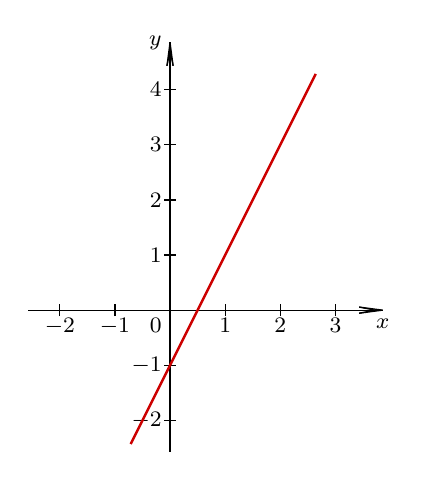
\begin{tikzpicture}
                        % \clip (0,0) rectangle (14.000000,10.000000);
                        {\footnotesize
                        
                        % Drawing 2D Cartesian system
                        \draw (3.000000,3.000000) node [anchor=north east] { $0$ };%
                        \draw [line width=0.016cm] (3.000000,2.925000) -- (3.000000,3.075000);%
                        \draw (3.700000,3.000000) node [anchor=north] { $1$ };%
                        \draw [line width=0.016cm] (3.700000,2.925000) -- (3.700000,3.075000);%
                        \draw (4.400000,3.000000) node [anchor=north] { $2$ };%
                        \draw [line width=0.016cm] (4.400000,2.925000) -- (4.400000,3.075000);%
                        \draw (5.100000,3.000000) node [anchor=north] { $3$ };%
                        \draw [line width=0.016cm] (5.100000,2.925000) -- (5.100000,3.075000);%
                        \draw (2.300000,3.000000) node [anchor=north] { $-1$ };%
                        \draw [line width=0.016cm] (2.300000,2.925000) -- (2.300000,3.075000);%
                        \draw (1.600000,3.000000) node [anchor=north] { $-2$ };%
                        \draw [line width=0.016cm] (1.600000,2.925000) -- (1.600000,3.075000);%
                        \draw (3.000000,3.700000) node [anchor=east] { $1$ };%
                        \draw [line width=0.016cm] (2.925000,3.700000) -- (3.075000,3.700000);%
                        \draw (3.000000,4.400000) node [anchor=east] { $2$ };%
                        \draw [line width=0.016cm] (2.925000,4.400000) -- (3.075000,4.400000);%
                        \draw (3.000000,5.100000) node [anchor=east] { $3$ };%
                        \draw [line width=0.016cm] (2.925000,5.100000) -- (3.075000,5.100000);%
                        \draw (3.000000,5.800000) node [anchor=east] { $4$ };%
                        \draw [line width=0.016cm] (2.925000,5.800000) -- (3.075000,5.800000);%
                        \draw (3.000000,2.300000) node [anchor=east] { $-1$ };%
                        \draw [line width=0.016cm] (2.925000,2.300000) -- (3.075000,2.300000);%
                        \draw (3.000000,1.600000) node [anchor=east] { $-2$ };%
                        \draw [line width=0.016cm] (2.925000,1.600000) -- (3.075000,1.600000);%
                        \draw (5.700000,3.000000) node [anchor=north] { $x$ };%
                        \draw (3.000000,6.400000) node [anchor=east] { $y$ };%
                        \draw [line width=0.016cm] (1.200000,3.000000) -- (5.700000,3.000000);%
                        \draw [line width=0.016cm] (5.402567,3.039158) -- (5.700000,3.000000);%
                        \draw [line width=0.016cm] (5.402567,3.039158) -- (5.600000,3.000000);%
                        \draw [line width=0.016cm] (5.402567,2.960842) -- (5.700000,3.000000);%
                        \draw [line width=0.016cm] (5.402567,2.960842) -- (5.600000,3.000000);%
                        \draw [line width=0.016cm] (3.000000,1.200000) -- (3.000000,6.400000);%
                        \draw [line width=0.016cm] (2.960842,6.102567) -- (3.000000,6.400000);%
                        \draw [line width=0.016cm] (2.960842,6.102567) -- (3.000000,6.300000);%
                        \draw [line width=0.016cm] (3.039158,6.102567) -- (3.000000,6.400000);%
                        \draw [line width=0.016cm] (3.039158,6.102567) -- (3.000000,6.300000);%
                        
                        % Changing color 204 0 0
                        \definecolor{r204g0b0}{rgb}{0.800000,0.000000,0.000000}%
                        \color{r204g0b0}% 
                        
                        % Drawing line l
                        \draw [line width=0.032cm] (2.500000,1.300000) -- (4.850000,6.000000);%
                        \color{black}
                        }
                        \end{tikzpicture}
                                                    
                \end{figure}

                \begin{figure}[H]
                    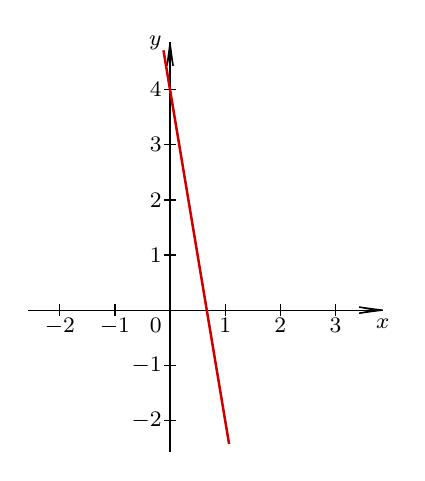
\begin{tikzpicture}
                        % \clip (0,0) rectangle (14.000000,10.000000);
                        {\footnotesize
                        
                        % Drawing 2D Cartesian system
                        \draw (3.000000,3.000000) node [anchor=north east] { $0$ };%
                        \draw [line width=0.016cm] (3.000000,2.925000) -- (3.000000,3.075000);%
                        \draw (3.700000,3.000000) node [anchor=north] { $1$ };%
                        \draw [line width=0.016cm] (3.700000,2.925000) -- (3.700000,3.075000);%
                        \draw (4.400000,3.000000) node [anchor=north] { $2$ };%
                        \draw [line width=0.016cm] (4.400000,2.925000) -- (4.400000,3.075000);%
                        \draw (5.100000,3.000000) node [anchor=north] { $3$ };%
                        \draw [line width=0.016cm] (5.100000,2.925000) -- (5.100000,3.075000);%
                        \draw (2.300000,3.000000) node [anchor=north] { $-1$ };%
                        \draw [line width=0.016cm] (2.300000,2.925000) -- (2.300000,3.075000);%
                        \draw (1.600000,3.000000) node [anchor=north] { $-2$ };%
                        \draw [line width=0.016cm] (1.600000,2.925000) -- (1.600000,3.075000);%
                        \draw (3.000000,3.700000) node [anchor=east] { $1$ };%
                        \draw [line width=0.016cm] (2.925000,3.700000) -- (3.075000,3.700000);%
                        \draw (3.000000,4.400000) node [anchor=east] { $2$ };%
                        \draw [line width=0.016cm] (2.925000,4.400000) -- (3.075000,4.400000);%
                        \draw (3.000000,5.100000) node [anchor=east] { $3$ };%
                        \draw [line width=0.016cm] (2.925000,5.100000) -- (3.075000,5.100000);%
                        \draw (3.000000,5.800000) node [anchor=east] { $4$ };%
                        \draw [line width=0.016cm] (2.925000,5.800000) -- (3.075000,5.800000);%
                        \draw (3.000000,2.300000) node [anchor=east] { $-1$ };%
                        \draw [line width=0.016cm] (2.925000,2.300000) -- (3.075000,2.300000);%
                        \draw (3.000000,1.600000) node [anchor=east] { $-2$ };%
                        \draw [line width=0.016cm] (2.925000,1.600000) -- (3.075000,1.600000);%
                        \draw (5.700000,3.000000) node [anchor=north] { $x$ };%
                        \draw (3.000000,6.400000) node [anchor=east] { $y$ };%
                        \draw [line width=0.016cm] (1.200000,3.000000) -- (5.700000,3.000000);%
                        \draw [line width=0.016cm] (5.402567,3.039158) -- (5.700000,3.000000);%
                        \draw [line width=0.016cm] (5.402567,3.039158) -- (5.600000,3.000000);%
                        \draw [line width=0.016cm] (5.402567,2.960842) -- (5.700000,3.000000);%
                        \draw [line width=0.016cm] (5.402567,2.960842) -- (5.600000,3.000000);%
                        \draw [line width=0.016cm] (3.000000,1.200000) -- (3.000000,6.400000);%
                        \draw [line width=0.016cm] (2.960842,6.102567) -- (3.000000,6.400000);%
                        \draw [line width=0.016cm] (2.960842,6.102567) -- (3.000000,6.300000);%
                        \draw [line width=0.016cm] (3.039158,6.102567) -- (3.000000,6.400000);%
                        \draw [line width=0.016cm] (3.039158,6.102567) -- (3.000000,6.300000);%
                        
                        % Changing color 204 0 0
                        \definecolor{r204g0b0}{rgb}{0.800000,0.000000,0.000000}%
                        \color{r204g0b0}% 
                        
                        % Drawing line l
                        \draw [line width=0.032cm] (3.750000,1.300000) -- (2.916667,6.300000);%
                        \color{black}
                        }
                        \end{tikzpicture}
                        
                \end{figure}

                \begin{figure}[H]
                    \begin{tikzpicture}
                        % \clip (0,0) rectangle (14.000000,10.000000);
                        {\footnotesize
                        
                        % Drawing 2D Cartesian system
                        \draw (3.000000,3.000000) node [anchor=north east] { $0$ };%
                        \draw [line width=0.016cm] (3.000000,2.925000) -- (3.000000,3.075000);%
                        \draw (3.700000,3.000000) node [anchor=north] { $1$ };%
                        \draw [line width=0.016cm] (3.700000,2.925000) -- (3.700000,3.075000);%
                        \draw (4.400000,3.000000) node [anchor=north] { $2$ };%
                        \draw [line width=0.016cm] (4.400000,2.925000) -- (4.400000,3.075000);%
                        \draw (5.100000,3.000000) node [anchor=north] { $3$ };%
                        \draw [line width=0.016cm] (5.100000,2.925000) -- (5.100000,3.075000);%
                        \draw (2.300000,3.000000) node [anchor=north] { $-1$ };%
                        \draw [line width=0.016cm] (2.300000,2.925000) -- (2.300000,3.075000);%
                        \draw (1.600000,3.000000) node [anchor=north] { $-2$ };%
                        \draw [line width=0.016cm] (1.600000,2.925000) -- (1.600000,3.075000);%
                        \draw (3.000000,3.700000) node [anchor=east] { $1$ };%
                        \draw [line width=0.016cm] (2.925000,3.700000) -- (3.075000,3.700000);%
                        \draw (3.000000,4.400000) node [anchor=east] { $2$ };%
                        \draw [line width=0.016cm] (2.925000,4.400000) -- (3.075000,4.400000);%
                        \draw (3.000000,5.100000) node [anchor=east] { $3$ };%
                        \draw [line width=0.016cm] (2.925000,5.100000) -- (3.075000,5.100000);%
                        \draw (3.000000,5.800000) node [anchor=east] { $4$ };%
                        \draw [line width=0.016cm] (2.925000,5.800000) -- (3.075000,5.800000);%
                        \draw (3.000000,2.300000) node [anchor=east] { $-1$ };%
                        \draw [line width=0.016cm] (2.925000,2.300000) -- (3.075000,2.300000);%
                        \draw (3.000000,1.600000) node [anchor=east] { $-2$ };%
                        \draw [line width=0.016cm] (2.925000,1.600000) -- (3.075000,1.600000);%
                        \draw (5.700000,3.000000) node [anchor=north] { $x$ };%
                        \draw (3.000000,6.400000) node [anchor=east] { $y$ };%
                        \draw [line width=0.016cm] (1.200000,3.000000) -- (5.700000,3.000000);%
                        \draw [line width=0.016cm] (5.402567,3.039158) -- (5.700000,3.000000);%
                        \draw [line width=0.016cm] (5.402567,3.039158) -- (5.600000,3.000000);%
                        \draw [line width=0.016cm] (5.402567,2.960842) -- (5.700000,3.000000);%
                        \draw [line width=0.016cm] (5.402567,2.960842) -- (5.600000,3.000000);%
                        \draw [line width=0.016cm] (3.000000,1.200000) -- (3.000000,6.400000);%
                        \draw [line width=0.016cm] (2.960842,6.102567) -- (3.000000,6.400000);%
                        \draw [line width=0.016cm] (2.960842,6.102567) -- (3.000000,6.300000);%
                        \draw [line width=0.016cm] (3.039158,6.102567) -- (3.000000,6.400000);%
                        \draw [line width=0.016cm] (3.039158,6.102567) -- (3.000000,6.300000);%
                        
                        % Changing color 204 0 0
                        \definecolor{r204g0b0}{rgb}{0.800000,0.000000,0.000000}%
                        \color{r204g0b0}% 
                        
                        % Drawing line l
                        \draw [line width=0.032cm] (4.900000,6.300000) -- (1.300000,2.700000);%
                        \color{black}
                        }
                        \end{tikzpicture}
                        
                \end{figure}


                \begin{figure}[H]
                    \begin{tikzpicture}
                        % \clip (0,0) rectangle (14.000000,10.000000);
                        {\footnotesize
                        
                        % Drawing 2D Cartesian system
                        \draw (3.000000,3.000000) node [anchor=north east] { $0$ };%
                        \draw [line width=0.016cm] (3.000000,2.925000) -- (3.000000,3.075000);%
                        \draw (3.700000,3.000000) node [anchor=north] { $1$ };%
                        \draw [line width=0.016cm] (3.700000,2.925000) -- (3.700000,3.075000);%
                        \draw (4.400000,3.000000) node [anchor=north] { $2$ };%
                        \draw [line width=0.016cm] (4.400000,2.925000) -- (4.400000,3.075000);%
                        \draw (5.100000,3.000000) node [anchor=north] { $3$ };%
                        \draw [line width=0.016cm] (5.100000,2.925000) -- (5.100000,3.075000);%
                        \draw (2.300000,3.000000) node [anchor=north] { $-1$ };%
                        \draw [line width=0.016cm] (2.300000,2.925000) -- (2.300000,3.075000);%
                        \draw (1.600000,3.000000) node [anchor=north] { $-2$ };%
                        \draw [line width=0.016cm] (1.600000,2.925000) -- (1.600000,3.075000);%
                        \draw (3.000000,3.700000) node [anchor=east] { $1$ };%
                        \draw [line width=0.016cm] (2.925000,3.700000) -- (3.075000,3.700000);%
                        \draw (3.000000,4.400000) node [anchor=east] { $2$ };%
                        \draw [line width=0.016cm] (2.925000,4.400000) -- (3.075000,4.400000);%
                        \draw (3.000000,5.100000) node [anchor=east] { $3$ };%
                        \draw [line width=0.016cm] (2.925000,5.100000) -- (3.075000,5.100000);%
                        \draw (3.000000,5.800000) node [anchor=east] { $4$ };%
                        \draw [line width=0.016cm] (2.925000,5.800000) -- (3.075000,5.800000);%
                        \draw (3.000000,2.300000) node [anchor=east] { $-1$ };%
                        \draw [line width=0.016cm] (2.925000,2.300000) -- (3.075000,2.300000);%
                        \draw (3.000000,1.600000) node [anchor=east] { $-2$ };%
                        \draw [line width=0.016cm] (2.925000,1.600000) -- (3.075000,1.600000);%
                        \draw (5.700000,3.000000) node [anchor=north] { $x$ };%
                        \draw (3.000000,6.400000) node [anchor=east] { $y$ };%
                        \draw [line width=0.016cm] (1.200000,3.000000) -- (5.700000,3.000000);%
                        \draw [line width=0.016cm] (5.402567,3.039158) -- (5.700000,3.000000);%
                        \draw [line width=0.016cm] (5.402567,3.039158) -- (5.600000,3.000000);%
                        \draw [line width=0.016cm] (5.402567,2.960842) -- (5.700000,3.000000);%
                        \draw [line width=0.016cm] (5.402567,2.960842) -- (5.600000,3.000000);%
                        \draw [line width=0.016cm] (3.000000,1.200000) -- (3.000000,6.400000);%
                        \draw [line width=0.016cm] (2.960842,6.102567) -- (3.000000,6.400000);%
                        \draw [line width=0.016cm] (2.960842,6.102567) -- (3.000000,6.300000);%
                        \draw [line width=0.016cm] (3.039158,6.102567) -- (3.000000,6.400000);%
                        \draw [line width=0.016cm] (3.039158,6.102567) -- (3.000000,6.300000);%
                        
                        % Changing color 204 0 0
                        \definecolor{r204g0b0}{rgb}{0.800000,0.000000,0.000000}%
                        \color{r204g0b0}% 
                        
                        % Drawing line l
                        \draw [line width=0.032cm] (1.300000,3.700000) -- (5.600000,3.700000);%
                        \color{black}
                        }
                        \end{tikzpicture}
                                                         
                \end{figure}


                \begin{figure}[H]
                    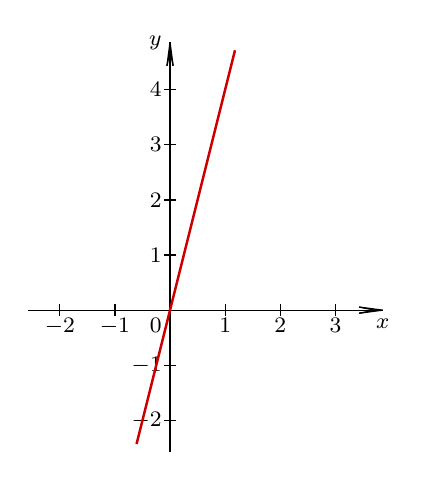
\begin{tikzpicture}
                        % \clip (0,0) rectangle (14.000000,10.000000);
                        {\footnotesize
                        
                        % Drawing 2D Cartesian system
                        \draw (3.000000,3.000000) node [anchor=north east] { $0$ };%
                        \draw [line width=0.016cm] (3.000000,2.925000) -- (3.000000,3.075000);%
                        \draw (3.700000,3.000000) node [anchor=north] { $1$ };%
                        \draw [line width=0.016cm] (3.700000,2.925000) -- (3.700000,3.075000);%
                        \draw (4.400000,3.000000) node [anchor=north] { $2$ };%
                        \draw [line width=0.016cm] (4.400000,2.925000) -- (4.400000,3.075000);%
                        \draw (5.100000,3.000000) node [anchor=north] { $3$ };%
                        \draw [line width=0.016cm] (5.100000,2.925000) -- (5.100000,3.075000);%
                        \draw (2.300000,3.000000) node [anchor=north] { $-1$ };%
                        \draw [line width=0.016cm] (2.300000,2.925000) -- (2.300000,3.075000);%
                        \draw (1.600000,3.000000) node [anchor=north] { $-2$ };%
                        \draw [line width=0.016cm] (1.600000,2.925000) -- (1.600000,3.075000);%
                        \draw (3.000000,3.700000) node [anchor=east] { $1$ };%
                        \draw [line width=0.016cm] (2.925000,3.700000) -- (3.075000,3.700000);%
                        \draw (3.000000,4.400000) node [anchor=east] { $2$ };%
                        \draw [line width=0.016cm] (2.925000,4.400000) -- (3.075000,4.400000);%
                        \draw (3.000000,5.100000) node [anchor=east] { $3$ };%
                        \draw [line width=0.016cm] (2.925000,5.100000) -- (3.075000,5.100000);%
                        \draw (3.000000,5.800000) node [anchor=east] { $4$ };%
                        \draw [line width=0.016cm] (2.925000,5.800000) -- (3.075000,5.800000);%
                        \draw (3.000000,2.300000) node [anchor=east] { $-1$ };%
                        \draw [line width=0.016cm] (2.925000,2.300000) -- (3.075000,2.300000);%
                        \draw (3.000000,1.600000) node [anchor=east] { $-2$ };%
                        \draw [line width=0.016cm] (2.925000,1.600000) -- (3.075000,1.600000);%
                        \draw (5.700000,3.000000) node [anchor=north] { $x$ };%
                        \draw (3.000000,6.400000) node [anchor=east] { $y$ };%
                        \draw [line width=0.016cm] (1.200000,3.000000) -- (5.700000,3.000000);%
                        \draw [line width=0.016cm] (5.402567,3.039158) -- (5.700000,3.000000);%
                        \draw [line width=0.016cm] (5.402567,3.039158) -- (5.600000,3.000000);%
                        \draw [line width=0.016cm] (5.402567,2.960842) -- (5.700000,3.000000);%
                        \draw [line width=0.016cm] (5.402567,2.960842) -- (5.600000,3.000000);%
                        \draw [line width=0.016cm] (3.000000,1.200000) -- (3.000000,6.400000);%
                        \draw [line width=0.016cm] (2.960842,6.102567) -- (3.000000,6.400000);%
                        \draw [line width=0.016cm] (2.960842,6.102567) -- (3.000000,6.300000);%
                        \draw [line width=0.016cm] (3.039158,6.102567) -- (3.000000,6.400000);%
                        \draw [line width=0.016cm] (3.039158,6.102567) -- (3.000000,6.300000);%
                        
                        % Changing color 204 0 0
                        \definecolor{r204g0b0}{rgb}{0.800000,0.000000,0.000000}%
                        \color{r204g0b0}% 
                        
                        % Drawing line l
                        \draw [line width=0.032cm] (2.575000,1.300000) -- (3.825000,6.300000);%
                        \color{black}
                        }
                        \end{tikzpicture}
                        
                \end{figure}


                \begin{figure}[H]
                    \begin{tikzpicture}
                        % \clip (0,0) rectangle (14.000000,10.000000);
                        {\footnotesize
                        
                        % Drawing 2D Cartesian system
                        \draw (3.000000,3.000000) node [anchor=north east] { $0$ };%
                        \draw [line width=0.016cm] (3.000000,2.925000) -- (3.000000,3.075000);%
                        \draw (3.700000,3.000000) node [anchor=north] { $1$ };%
                        \draw [line width=0.016cm] (3.700000,2.925000) -- (3.700000,3.075000);%
                        \draw (4.400000,3.000000) node [anchor=north] { $2$ };%
                        \draw [line width=0.016cm] (4.400000,2.925000) -- (4.400000,3.075000);%
                        \draw (5.100000,3.000000) node [anchor=north] { $3$ };%
                        \draw [line width=0.016cm] (5.100000,2.925000) -- (5.100000,3.075000);%
                        \draw (2.300000,3.000000) node [anchor=north] { $-1$ };%
                        \draw [line width=0.016cm] (2.300000,2.925000) -- (2.300000,3.075000);%
                        \draw (1.600000,3.000000) node [anchor=north] { $-2$ };%
                        \draw [line width=0.016cm] (1.600000,2.925000) -- (1.600000,3.075000);%
                        \draw (3.000000,3.700000) node [anchor=east] { $1$ };%
                        \draw [line width=0.016cm] (2.925000,3.700000) -- (3.075000,3.700000);%
                        \draw (3.000000,4.400000) node [anchor=east] { $2$ };%
                        \draw [line width=0.016cm] (2.925000,4.400000) -- (3.075000,4.400000);%
                        \draw (3.000000,5.100000) node [anchor=east] { $3$ };%
                        \draw [line width=0.016cm] (2.925000,5.100000) -- (3.075000,5.100000);%
                        \draw (3.000000,5.800000) node [anchor=east] { $4$ };%
                        \draw [line width=0.016cm] (2.925000,5.800000) -- (3.075000,5.800000);%
                        \draw (3.000000,2.300000) node [anchor=east] { $-1$ };%
                        \draw [line width=0.016cm] (2.925000,2.300000) -- (3.075000,2.300000);%
                        \draw (3.000000,1.600000) node [anchor=east] { $-2$ };%
                        \draw [line width=0.016cm] (2.925000,1.600000) -- (3.075000,1.600000);%
                        \draw (5.700000,3.000000) node [anchor=north] { $x$ };%
                        \draw (3.000000,6.400000) node [anchor=east] { $y$ };%
                        \draw [line width=0.016cm] (1.200000,3.000000) -- (5.700000,3.000000);%
                        \draw [line width=0.016cm] (5.402567,3.039158) -- (5.700000,3.000000);%
                        \draw [line width=0.016cm] (5.402567,3.039158) -- (5.600000,3.000000);%
                        \draw [line width=0.016cm] (5.402567,2.960842) -- (5.700000,3.000000);%
                        \draw [line width=0.016cm] (5.402567,2.960842) -- (5.600000,3.000000);%
                        \draw [line width=0.016cm] (3.000000,1.200000) -- (3.000000,6.400000);%
                        \draw [line width=0.016cm] (2.960842,6.102567) -- (3.000000,6.400000);%
                        \draw [line width=0.016cm] (2.960842,6.102567) -- (3.000000,6.300000);%
                        \draw [line width=0.016cm] (3.039158,6.102567) -- (3.000000,6.400000);%
                        \draw [line width=0.016cm] (3.039158,6.102567) -- (3.000000,6.300000);%
                        
                        % Changing color 204 0 0
                        \definecolor{r204g0b0}{rgb}{0.800000,0.000000,0.000000}%
                        \color{r204g0b0}% 
                        
                        % Drawing line l
                        \draw [line width=0.032cm] (2.700000,1.300000) -- (5.600000,4.200000);%
                        \color{black}
                        }
                        \end{tikzpicture}
                        
                \end{figure}



                \begin{figure}[H]
                    \begin{tikzpicture}
                        % \clip (0,0) rectangle (14.000000,10.000000);
                        {\footnotesize
                        
                        % Drawing 2D Cartesian system
                        \draw (3.000000,3.000000) node [anchor=north east] { $0$ };%
                        \draw [line width=0.016cm] (3.000000,2.925000) -- (3.000000,3.075000);%
                        \draw (3.700000,3.000000) node [anchor=north] { $1$ };%
                        \draw [line width=0.016cm] (3.700000,2.925000) -- (3.700000,3.075000);%
                        \draw (4.400000,3.000000) node [anchor=north] { $2$ };%
                        \draw [line width=0.016cm] (4.400000,2.925000) -- (4.400000,3.075000);%
                        \draw (5.100000,3.000000) node [anchor=north] { $3$ };%
                        \draw [line width=0.016cm] (5.100000,2.925000) -- (5.100000,3.075000);%
                        \draw (2.300000,3.000000) node [anchor=north] { $-1$ };%
                        \draw [line width=0.016cm] (2.300000,2.925000) -- (2.300000,3.075000);%
                        \draw (1.600000,3.000000) node [anchor=north] { $-2$ };%
                        \draw [line width=0.016cm] (1.600000,2.925000) -- (1.600000,3.075000);%
                        \draw (3.000000,3.700000) node [anchor=east] { $1$ };%
                        \draw [line width=0.016cm] (2.925000,3.700000) -- (3.075000,3.700000);%
                        \draw (3.000000,4.400000) node [anchor=east] { $2$ };%
                        \draw [line width=0.016cm] (2.925000,4.400000) -- (3.075000,4.400000);%
                        \draw (3.000000,5.100000) node [anchor=east] { $3$ };%
                        \draw [line width=0.016cm] (2.925000,5.100000) -- (3.075000,5.100000);%
                        \draw (3.000000,5.800000) node [anchor=east] { $4$ };%
                        \draw [line width=0.016cm] (2.925000,5.800000) -- (3.075000,5.800000);%
                        \draw (3.000000,2.300000) node [anchor=east] { $-1$ };%
                        \draw [line width=0.016cm] (2.925000,2.300000) -- (3.075000,2.300000);%
                        \draw (3.000000,1.600000) node [anchor=east] { $-2$ };%
                        \draw [line width=0.016cm] (2.925000,1.600000) -- (3.075000,1.600000);%
                        \draw (5.700000,3.000000) node [anchor=north] { $x$ };%
                        \draw (3.000000,6.400000) node [anchor=east] { $y$ };%
                        \draw [line width=0.016cm] (1.200000,3.000000) -- (5.700000,3.000000);%
                        \draw [line width=0.016cm] (5.402567,3.039158) -- (5.700000,3.000000);%
                        \draw [line width=0.016cm] (5.402567,3.039158) -- (5.600000,3.000000);%
                        \draw [line width=0.016cm] (5.402567,2.960842) -- (5.700000,3.000000);%
                        \draw [line width=0.016cm] (5.402567,2.960842) -- (5.600000,3.000000);%
                        \draw [line width=0.016cm] (3.000000,1.200000) -- (3.000000,6.400000);%
                        \draw [line width=0.016cm] (2.960842,6.102567) -- (3.000000,6.400000);%
                        \draw [line width=0.016cm] (2.960842,6.102567) -- (3.000000,6.300000);%
                        \draw [line width=0.016cm] (3.039158,6.102567) -- (3.000000,6.400000);%
                        \draw [line width=0.016cm] (3.039158,6.102567) -- (3.000000,6.300000);%
                        
                        % Changing color 204 0 0
                        \definecolor{r204g0b0}{rgb}{0.800000,0.000000,0.000000}%
                        \color{r204g0b0}% 
                        
                        % Drawing line l
                        \draw [line width=0.032cm] (1.300000,3.550000) -- (5.600000,5.700000);%
                        \color{black}
                        }
                        \end{tikzpicture}
                                              
                \end{figure}


                \begin{figure}[H]
                    \begin{tikzpicture}
                        % \clip (0,0) rectangle (14.000000,10.000000);
                        {\footnotesize
                        
                        % Drawing 2D Cartesian system
                        \draw (3.000000,3.000000) node [anchor=north east] { $0$ };%
                        \draw [line width=0.016cm] (3.000000,2.925000) -- (3.000000,3.075000);%
                        \draw (3.700000,3.000000) node [anchor=north] { $1$ };%
                        \draw [line width=0.016cm] (3.700000,2.925000) -- (3.700000,3.075000);%
                        \draw (4.400000,3.000000) node [anchor=north] { $2$ };%
                        \draw [line width=0.016cm] (4.400000,2.925000) -- (4.400000,3.075000);%
                        \draw (5.100000,3.000000) node [anchor=north] { $3$ };%
                        \draw [line width=0.016cm] (5.100000,2.925000) -- (5.100000,3.075000);%
                        \draw (2.300000,3.000000) node [anchor=north] { $-1$ };%
                        \draw [line width=0.016cm] (2.300000,2.925000) -- (2.300000,3.075000);%
                        \draw (1.600000,3.000000) node [anchor=north] { $-2$ };%
                        \draw [line width=0.016cm] (1.600000,2.925000) -- (1.600000,3.075000);%
                        \draw (3.000000,3.700000) node [anchor=east] { $1$ };%
                        \draw [line width=0.016cm] (2.925000,3.700000) -- (3.075000,3.700000);%
                        \draw (3.000000,4.400000) node [anchor=east] { $2$ };%
                        \draw [line width=0.016cm] (2.925000,4.400000) -- (3.075000,4.400000);%
                        \draw (3.000000,5.100000) node [anchor=east] { $3$ };%
                        \draw [line width=0.016cm] (2.925000,5.100000) -- (3.075000,5.100000);%
                        \draw (3.000000,5.800000) node [anchor=east] { $4$ };%
                        \draw [line width=0.016cm] (2.925000,5.800000) -- (3.075000,5.800000);%
                        \draw (3.000000,2.300000) node [anchor=east] { $-1$ };%
                        \draw [line width=0.016cm] (2.925000,2.300000) -- (3.075000,2.300000);%
                        \draw (3.000000,1.600000) node [anchor=east] { $-2$ };%
                        \draw [line width=0.016cm] (2.925000,1.600000) -- (3.075000,1.600000);%
                        \draw (5.700000,3.000000) node [anchor=north] { $x$ };%
                        \draw (3.000000,6.400000) node [anchor=east] { $y$ };%
                        \draw [line width=0.016cm] (1.200000,3.000000) -- (5.700000,3.000000);%
                        \draw [line width=0.016cm] (5.402567,3.039158) -- (5.700000,3.000000);%
                        \draw [line width=0.016cm] (5.402567,3.039158) -- (5.600000,3.000000);%
                        \draw [line width=0.016cm] (5.402567,2.960842) -- (5.700000,3.000000);%
                        \draw [line width=0.016cm] (5.402567,2.960842) -- (5.600000,3.000000);%
                        \draw [line width=0.016cm] (3.000000,1.200000) -- (3.000000,6.400000);%
                        \draw [line width=0.016cm] (2.960842,6.102567) -- (3.000000,6.400000);%
                        \draw [line width=0.016cm] (2.960842,6.102567) -- (3.000000,6.300000);%
                        \draw [line width=0.016cm] (3.039158,6.102567) -- (3.000000,6.400000);%
                        \draw [line width=0.016cm] (3.039158,6.102567) -- (3.000000,6.300000);%
                        
                        % Changing color 204 0 0
                        \definecolor{r204g0b0}{rgb}{0.800000,0.000000,0.000000}%
                        \color{r204g0b0}% 
                        
                        % Drawing line l
                        \draw [line width=0.032cm] (4.700000,1.300000) -- (1.300000,4.700000);%
                        \color{black}
                        }
                        \end{tikzpicture}
                        
                \end{figure}


                \begin{figure}[H]
                    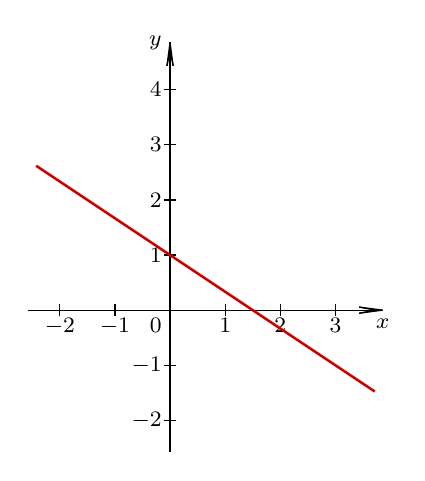
\begin{tikzpicture}
                        % \clip (0,0) rectangle (14.000000,10.000000);
                        {\footnotesize
                        
                        % Drawing 2D Cartesian system
                        \draw (3.000000,3.000000) node [anchor=north east] { $0$ };%
                        \draw [line width=0.016cm] (3.000000,2.925000) -- (3.000000,3.075000);%
                        \draw (3.700000,3.000000) node [anchor=north] { $1$ };%
                        \draw [line width=0.016cm] (3.700000,2.925000) -- (3.700000,3.075000);%
                        \draw (4.400000,3.000000) node [anchor=north] { $2$ };%
                        \draw [line width=0.016cm] (4.400000,2.925000) -- (4.400000,3.075000);%
                        \draw (5.100000,3.000000) node [anchor=north] { $3$ };%
                        \draw [line width=0.016cm] (5.100000,2.925000) -- (5.100000,3.075000);%
                        \draw (2.300000,3.000000) node [anchor=north] { $-1$ };%
                        \draw [line width=0.016cm] (2.300000,2.925000) -- (2.300000,3.075000);%
                        \draw (1.600000,3.000000) node [anchor=north] { $-2$ };%
                        \draw [line width=0.016cm] (1.600000,2.925000) -- (1.600000,3.075000);%
                        \draw (3.000000,3.700000) node [anchor=east] { $1$ };%
                        \draw [line width=0.016cm] (2.925000,3.700000) -- (3.075000,3.700000);%
                        \draw (3.000000,4.400000) node [anchor=east] { $2$ };%
                        \draw [line width=0.016cm] (2.925000,4.400000) -- (3.075000,4.400000);%
                        \draw (3.000000,5.100000) node [anchor=east] { $3$ };%
                        \draw [line width=0.016cm] (2.925000,5.100000) -- (3.075000,5.100000);%
                        \draw (3.000000,5.800000) node [anchor=east] { $4$ };%
                        \draw [line width=0.016cm] (2.925000,5.800000) -- (3.075000,5.800000);%
                        \draw (3.000000,2.300000) node [anchor=east] { $-1$ };%
                        \draw [line width=0.016cm] (2.925000,2.300000) -- (3.075000,2.300000);%
                        \draw (3.000000,1.600000) node [anchor=east] { $-2$ };%
                        \draw [line width=0.016cm] (2.925000,1.600000) -- (3.075000,1.600000);%
                        \draw (5.700000,3.000000) node [anchor=north] { $x$ };%
                        \draw (3.000000,6.400000) node [anchor=east] { $y$ };%
                        \draw [line width=0.016cm] (1.200000,3.000000) -- (5.700000,3.000000);%
                        \draw [line width=0.016cm] (5.402567,3.039158) -- (5.700000,3.000000);%
                        \draw [line width=0.016cm] (5.402567,3.039158) -- (5.600000,3.000000);%
                        \draw [line width=0.016cm] (5.402567,2.960842) -- (5.700000,3.000000);%
                        \draw [line width=0.016cm] (5.402567,2.960842) -- (5.600000,3.000000);%
                        \draw [line width=0.016cm] (3.000000,1.200000) -- (3.000000,6.400000);%
                        \draw [line width=0.016cm] (2.960842,6.102567) -- (3.000000,6.400000);%
                        \draw [line width=0.016cm] (2.960842,6.102567) -- (3.000000,6.300000);%
                        \draw [line width=0.016cm] (3.039158,6.102567) -- (3.000000,6.400000);%
                        \draw [line width=0.016cm] (3.039158,6.102567) -- (3.000000,6.300000);%
                        
                        % Changing color 204 0 0
                        \definecolor{r204g0b0}{rgb}{0.800000,0.000000,0.000000}%
                        \color{r204g0b0}% 
                        
                        % Drawing line l
                        \draw [line width=0.032cm] (1.300000,4.833220) -- (5.600000,1.966840);%
                        \color{black}
                        }
                        \end{tikzpicture}
                        
                \end{figure}


            \end{multicols}

        \end{naloga}

    



            \begin{naloga}
                Narišite graf sestavljene funkcije in zapišite njeno zalogo vrednosti.
                    \begin{multicols}{2}
                    \begin{itemize}
                        \item $f(x)=\begin{cases}
                            2x; & x\leq 2 \\ 4; &x>2
                        \end{cases}$ \\~
                        \item $g(x)=\begin{cases}
                            x+3; & x\leq -2 \\ -x-1; &x>-2
                        \end{cases}$ \\~
                        \item $h(x)=\begin{cases}
                            x; & x\leq 1 \\ -1; & x>1
                        \end{cases}$ \\~
                        \item $k(x)=\begin{cases}
                            -x+1; & x\leq 2 \\ -1; &2<x<4 \\ x-5; &x\geq 4
                        \end{cases}$ \\~
                        \item $l(x)=\begin{cases}
                            0.5x; & x\leq 2 \\ 2x-3; &2<x<4 \\ 0.5x+3; &x\geq 4
                        \end{cases}$ \\~
                    \end{itemize}
                \end{multicols}
        \end{naloga}


        \begin{naloga}
                Narišite graf funkcije. 
                \begin{multicols}{2}
                    \begin{itemize}
                        \item $f(x)=|3x-3|$ 
                        \item $g(x)=|2x+1|+1$ 
                        \item $h(x)=1-|x+1|$ 
                        \item $i(x)=3-|2x-1|$ 
                        \item $j(x)=x+|x-2|$ 
                        \item $k(x)=|x+1|-2$ 
                        \item $l(x)=-|0.5x+3|$ 
                        \item $m(x)=3-|x-2|$ 
                    \end{itemize}
                \end{multicols}
        \end{naloga}




\end{priprava}